\subsection{Queue}
\paragraph{} This simulation's module represents the queue, that should be one for each till or one for all. In the second case, the queue is "first in first out". Through the decisor, the customers are sent to the tills. 
\begin{figure}[h]
  \begin{center}
  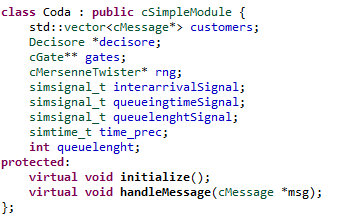
\includegraphics[width=80mm]{queue.png}
  \caption{Queue.}
  \label{fig:que}
  \end{center}
\end{figure}

\paragraph{initialize} This function will initialize all the port gates of Coda, because it need as many output ports as the number of Casse in the simulation. Then the simulation will start.

\paragraph{handleMessage} This function manages the queue: it checks if a new customer is arrived, if there is at least one customer in the queue and there is at least one available till, it sends the customer to the till.
